\documentclass{article}
\usepackage[utf8]{inputenc}
\usepackage{graphicx}
\usepackage{amsmath}
\usepackage{caption}
\usepackage{hyperref}
\usepackage{geometry}
\geometry{margin=2.5cm}

\title{Percolation Project}
\author{Anaya Lizarazo, Bryan Johan; Pinilla Correa, Santiago \& Torres Otálora, Erick}
\date{\today}

\begin{document} 

\maketitle

\section{Introducción}
Intro.

\section{Resultados}
Aquí una figura de ejemplo:

\begin{figure}[h]
    \centering
    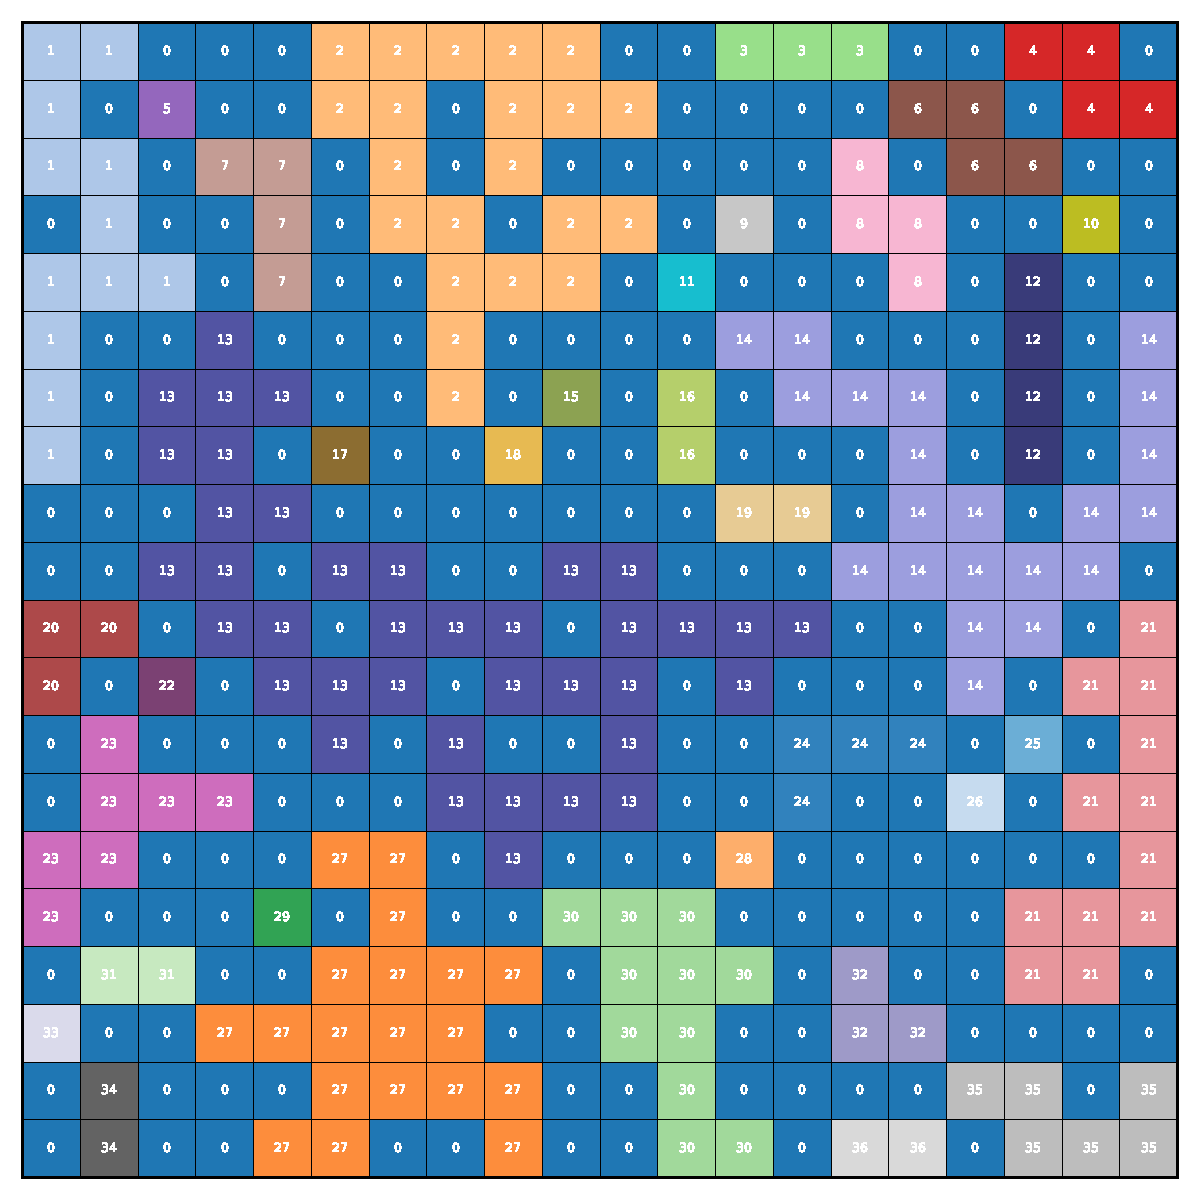
\includegraphics[width=0.6\textwidth]{clusters.pdf}
    \caption{Gráfica generada con Python.}
\end{figure}



\section{Conclusiones}
...

\end{document}
